% Setup - do not change
\documentclass[11pt]{article}
\usepackage[top=0.9in, left=0.9in, bottom=0.9in, right=0.9in]{geometry} 
\usepackage{parskip}

\usepackage[english]{babel}
\usepackage[utf8]{inputenc}
\usepackage{amsmath,amsthm,amssymb,graphicx,pdfpages,lipsum,hyperref}
\usepackage[none]{hyphenat}
\usepackage{csquotes}

\setlength\parindent{0pt}
%%%%%%%%%%%%%%%%%%%%%%%%%%%%%%%%%%%%%%%%%%%%%%%%%%%%%%%%%%%%%%%%%%%
% add other packages here if required

%% Bibliography are specified in this file. You can also choose inline bib style if you want to. But make sure your citation style is consistent (and proper)
% For more details on citation: https://library.unimelb.edu.au/recite
\usepackage[sorting = none]{biblatex}
\addbibresource{references.bib}
\usepackage{graphicx}

%%%%%%%%%%%%%%%%%%%%%%%%%%%%%%%%%%%%%%%%%%%%%%%%%%%%%%%%%%%%%%%%%%% the '%' symbol denotes comments

% Begin document creation
% DELETE THE \lipsum PLACEHOLDERS WHEN YOU BEGIN
\title{\textbf{Determining Demand for Yellow Taxis in New York City} \\ }
\author{
Aryan Shahi \\
Student ID: 1170385 \\
%% Replace the link with your github repo
% 1. Remember to escape underscore in the link.
% 2. Remember to include the commit you want to submit in the link
\href{https://github.com/MAST30034-Applied-Data-Science/mast30034-project-1-AryanShahi20}{Github repo with commit}
}

\begin{document}
\maketitle

\section{Introduction}
A huge problem for yellow taxi-cab drivers in New York city is the wastage of time in-between fairs. Being the only cab that can be street hailed, these drivers drive around looking for passengers or let precious time pass by as they park their cars and await an e-hail. This report seeks to reduce this in-between waiting time by analysing taxi trip data to reliably predict the number of pickups a cabby can expect in a given location, at any given hour, throughout the year. This modelling is done with decision trees and the model is built on a combination of useful features from two datasets (see 1.1). The aim is to find the best locations and time periods where cab drivers can consistently find passengers to maximize their daily profits.

The target audience of this paper is yellow taxi drivers in NYC and those associated with managing their deployment i.e., the taxi and limousine commission (TLC). It is in their best interest to strategically plan out the number of taxis that should be in each location given demand. This allows taxi drivers to earn a liveable income through consistent fares and makes it so that their fares don’t clash with other taxis or for hire vehicles (FHVs).

\subsection{Datasets}
The first dataset used is the 2019 yellow taxi dataset from New York City Taxi and Limousine Commission \cite{TLC}. The dataset has 84,598,444 rows and 19 columns with each row representing a single journey taken in a cab whilst the columns represent features such as pick up location and trip distance. Yellow taxis were chosen because the drivers are more likely to have only one job whereas FHV drivers generally work multiple jobs. 2019 was chosen as it was the most recent year which wasn’t affected by COVID lockdowns and restrictions. All of 2019 was chosen so trends between different months could be observed.

The second dataset used is the 2019 NYC weather observation data from IOWA state university \cite{weather} with the reason being that there should be a greater demand for taxi pickups in adverse weather conditions such as rain. The dataset is composed of 8368 rows and 30 columns with each row representing observations for a given hour in the year whilst the columns represent features such as wind speed and temperature. The measurements all happened in one spot (JRB station Manhattan), so the model assumes these measurements are similar for all locations in NYC. 

Model testing was done with data from January and February of 2020 because March was when the first COVID case was detected in NYC. March onwards was not used as there would be inconsistent variations in demand due to COVID-19 which would skew model evaluation.

\section{Preprocessing and Outliers}
 Starting with the weather dataset, the first step was the removal of unnecessary features that would not have any correlation with demand in a given location, at a given hour, throughout the year. This resulted in the removal of 25 columns of which some were mostly filled with null values whilst others were useless e.g., sea level pressure. The 5 remaining columns didn't have any NULL values, so no imputations or removals were required. The remaining columns were renamed for clarity and the timestamp column was used to extract the month, day, and hour for analysis.
 
Useless columns were also removed from the taxi dataset due to having no correlation with demand. They included features like passenger count and payment type. The timestamp format was changed to the same one as the weather dataset so they could be inner joined in the future. A journey time column was created by subtracting pickup time from drop off time to filter out unhelpful instances. The aim of this report is to reduce waiting time and increase a cabbies daily profits by finding points with high demand. High demand makes no difference if the cabby is doing 2-minute journeys and then waiting 2 minutes for their next passenger as it’s like doing 20-minute journeys and then waiting 20 minutes for a new passenger. Therefore, Journey time less then 10 minutes was filtered out to truly determine the best points with high demand. This removed 36,828,914 entries. Rows with trip distance equal to or less than 0 were also removed which got rid of a further 121,536 entries. No rows contained any NULL values, so no imputations or removals were required. Counts were aggregated by month, day, hour, and location id. This dataset was merged with the weather dataset.

Using inner join to merge the datasets further removed 48,204 entries from rows that were outside the 2019 time period. The final merged data set contained 1,032,570 rows and 9 feature’s including location, count, temperature, dew point temperature, humidity, wind speed, month, day, and pickup hour.



\section{Analysis}

\subsection{Hour}

\begin{figure}[h]
    % change the scale multiplier to make the figures smaller or larger
    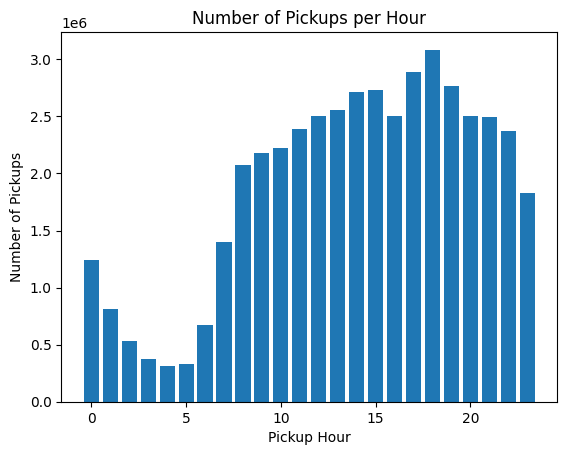
\includegraphics[width=0.55\textwidth]{plots/hour.png}
    % this ensures your figures are centered where possible
    \centering
    \caption{Total number of yellow cab pickups for each hour in 2019} % refer to this image as (Figure 1)
\end{figure}

It is instantly evident that the pickup hour plays a huge role in demand. Obviously 1 to 6 am would have the lowest number of pickups as most people are asleep and the only people needing yellow cabs at that time are arrivals from the airport and partiers. There also won’t be as many cabs patrolling the streets at those times either. One way ANOVA between hour and pickups yields a p-value of 3.4e-13 which shows that pickup hour is significant. There seems to be a slight negative skew in the graph. The highest demand was at 6 pm with 3.08 million pickups which is assumed to be due to dinner time. The lowest demand was at 4 am with only 0.31 million pickups which is 10x less. The best time for cabbies who plan to work only a few hours would be from 2pm to 7pm.

\subsection{Day}

\begin{figure}[h]
    % change the scale multiplier to make the figures smaller or larger
    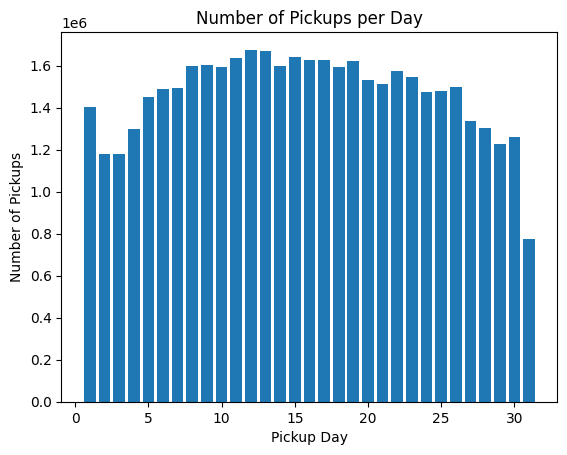
\includegraphics[width=0.4\textwidth]{plots/day.png}
    % this ensures your figures are centered where possible
    \centering
    \caption{Total number of yellow cab pickups for each day of the month in 2019} % refer to this image as (Figure 1)
\end{figure}

At first glance the data is spread out in a bell curve with the greatest number of pickups (demand) in the middle and the lowest number at the edges. Day 1 seems to be an outlier and its obvious why day 31 has the lowest demand as not all months have it. The day seems to have an impact on demand. One way ANOVA analysis between day and pickups yielded a p-value of 5.3e-36 showing that pickup day is significant. The best day for demand was the 12th with 1.68 million pickups and the worst was the 31st with only 0.77 million. For cabbies looking to work only a few days, the best days would be days 8 to 19.

\subsection{Month}

\begin{figure}[h]
    % change the scale multiplier to make the figures smaller or larger
    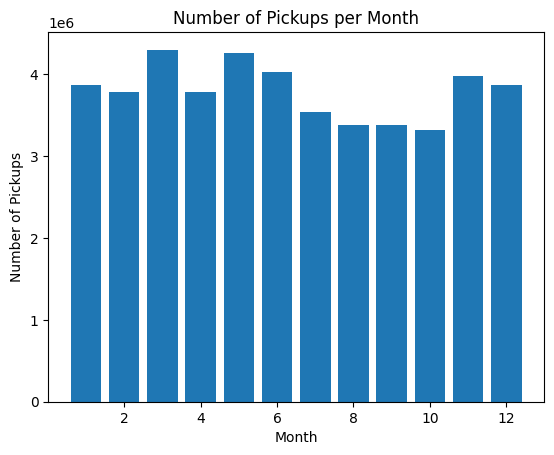
\includegraphics[width=0.4\textwidth]{plots/month.png}
    % this ensures your figures are centered where possible
    \centering
    \caption{Total number of yellow cab pickups for each day of the month in 2019} % refer to this image as (Figure 1)
\end{figure}

The most demanding month was March with 4.3 million pickups and the least demanding month was October with 3.3 million pickups. It was interesting to see February not be the least demanding considering it only had 28 days in 2019. One way ANOVA between number of pickups and month yielded a p-value of 5.5e-22 making month statistically significant. Cabbies that plan to work only a few months should choose March, May, June, November, and December.

\subsection{Location}

\begin{figure}[h]
    % change the scale multiplier to make the figures smaller or larger
    \includegraphics[width=0.8\textwidth]{plots/map.png}
    % this ensures your figures are centered where possible
    \centering
    \caption{Total number of yellow cab pickups for each location id region in NYC in 2019} % refer to this image as (Figure 1)
\end{figure}

Instantly we can see that pickup location id plays a huge role on demand. A one-way ANOVA between id and number of pickups gives a p-value of 1.8e-11 which shows that it is statistically significant. Most of the regions are at the lower end of the spectrum with a minor number of pickups compared to the 3 “colourful” sections. The highest demand is in the colourful section at the bottom right. This is region 132 and the high demand here is explained by it containing JFK airport. The pink colourful section northwest of it (region 138) contains LaGuardia airport. The final colourful section to the west of 138 doesn’t have any airports but is one of the most densely populated sections in NYC and is contained within Manhattan. Cabbies that want a steady supply of customers should go to one of the three colourful sections with Manhattan being the best.

\subsection{Weather and Interaction}

\begin{figure}[h]
    % change the scale multiplier to make the figures smaller or larger
    
\includegraphics[width=0.5\textwidth]{plots/weather.png}
    % this ensures your figures are centered where possible
    \centering
    \caption{Pearson correlation for training dataset} % refer to this image as (Figure 1)
\end{figure}

Looking at figure 5 below, the dependent variable (count) has the biggest correlation with pickup hour. The second biggest correlation is with pick up location id but that should be disregarded here as location id is a nominal variable. It’s interesting to see that month is adequately correlated with temperature which is to be expected. Out of all the weather features, the one that count is correlated with the most is wind speed. It was expected that temperature would have a stronger relationship with count, but this was not the case. Relative humidity and dew point temperature have the worst correlation with count so they will be removed. Coincidentally, they both have a strong correlation with each other. The main reason why weather variables are not as correlated with count is because there is so much variation in count which makes it harder to predict.

\section{Statistical Modelling}
The two models being used to predict the pickup count in a given location, at any given hour, throughout the year, are decision trees and random Forrest. Random forest is simply a decision tree ensemble and claimed to generally be more accurate than a decision tree so it will be interesting to see how they perform compared to each other. The reason for choosing two decision tree-based models was made as the data is composed of lots of good categorical feature such as pickup hour, location id etc. which can form a solid basis for splitting and lead to better predictions.

\subsection{Decision Tree}

\begin{figure}[h]
    % change the scale multiplier to make the figures smaller or larger
    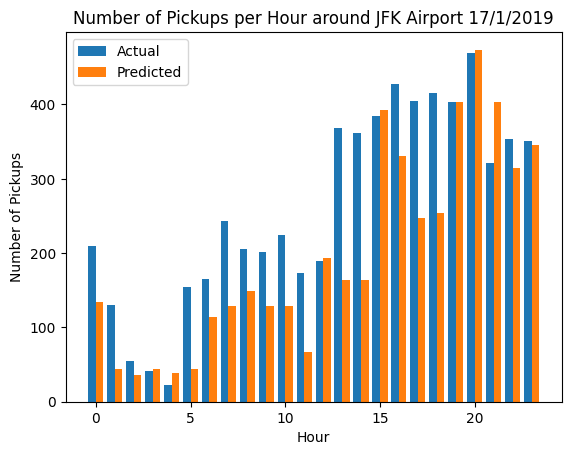
\includegraphics[width=0.6\textwidth]{plots/tree.png}
    % this ensures your figures are centered where possible
    \centering
    \caption{Combined bar chart showing predictions vs actual for a random day} % refer to this image as (Figure 1)
\end{figure}

The decision tree model was trained on location id, month, day, hour, temp, and wind speed. In terms of hyperparameter tuning, max depth was 12 and max bins were 263. Depth would have been higher if computational power allowed it as model accuracy was consistently increasing going from a depth of 1 to 12. Max bins were set at 263 because that’s the number of unique pick-up location ids. The figure above shows that the model performed very well for a random location-month-day-hour combination. The predicted values for each hour are very close to the actual values. The model mainly seems to underestimate except for the outlier at hour 21. Its better for the model to underestimate then overestimate in this situation. The evaluation metric used was mean absolute error as it would indicate how far off on average the model was from the correct number of pickups. The decision tree achieved a mean absolute error of 16.57 over the whole train set which, when compared with the pickup count mean of 40.2 and standard deviation of 77.2, is a good score.

\subsection{Random Forrest}

\begin{figure}[h]
    % change the scale multiplier to make the figures smaller or larger
    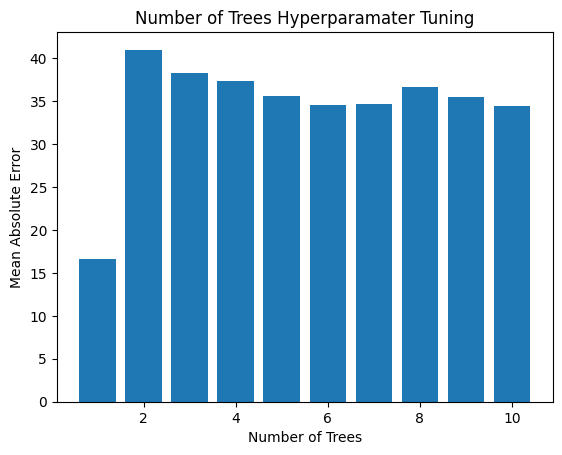
\includegraphics[width=0.7\textwidth]{plots/param.png}
    % this ensures your figures are centered where possible
    \centering
    \caption{Mean absolute errors for random forests with different numbers of trees} % refer to this image as (Figure 1)
\end{figure}

The random forest model was trained on the same set of features as the decision tree. Hyperparameters max depth and max bins were also kept the same to get the best comparison. We can see from figure 7, the random forest model performed best when it only had one tree making it similar to a decision tree model. As soon as the number of trees went past 1 the mean absolute error doubled and remained at that level despite increasing the number of trees. This was an interesting find as random forests are said to have higher accuracy cause the combine many trees. A reason why it performed so poorly with multiple trees could be due to the high variance in counts or the fact that multiple trees are built using bagging and feature randomness which messes with the structure of having one count per location-month-day-hour. It is safe to say that a single decision tree is better with this type of training set.

\section{Discussion}
A key thing to remember is that this analysis was based on determining the demand at any given hour-day-month-pickup location for journeys that would last over 10 minutes. This means that all under 10-minute journeys were removed from both the training and test sets (see reasoning in section 2). From both the analysis and the model it can be seen that there are definitely key factors that can help determine the number of pickups you can expect to have at a given location during any hour throughout the year. 

A recommendation to yellow taxicab drivers is to carefully think about when/where they drive since it does matter significantly as shown in this report. For example, waiting at the JFK airport for passengers has a 10x greater chance of getting a fare then most of the regions in New York. Driving during lunchtime will mean having to wait longer in between fares when compared to driving during dinner time. There are other factors at play here such as how busy a location is, so the best course of action is to try and determine through trial and error what works best.

A recommendation to the TLC is to build a model similar to this for their own use. The TLC overlooks yellow cabs, green cabs, and ridesharing vehicles in NYC so something like this is crucial. It would mean that there is better coordination between all these drivers which would allow everyone to get an equal share from fares by the end of the day. This report has shown that there are huge differences in demand between different times and locations. Using a model that predicts demand similarly to the decision tree would allow for optimal allocation of drivers to each of the 263 regions.

Future improvements would be to include more data, both from different years and different types of vehicles. This wasn’t possible in this analysis due to computational power. Exploring other types of models and combining datasets such as sporting events and borough populations over time could help make a better predictor for demand. COVID datasets should be taken into consideration too for making models based on more current years.


\clearpage

% BEGIN REFERENCES SECTION
\printbibliography

\end{document}